\section{Testing}
Il testing delle API è stato fatto tutto all'interno di un unico file chiamato 'test.js'. È possibile trovare questo file nella root della cartella di Back-end. I test che sono stati fatti sono abbastanza banali, in quanto si è verificato che soltanto lo 'statusCode' e qualche volta il campo 'message' presente all'interno della risposta fossero corretti. Ad esempio per l'API di registrazione sono stati impostati i seguenti casi di test:

\begin{figure}[!h]
\centering
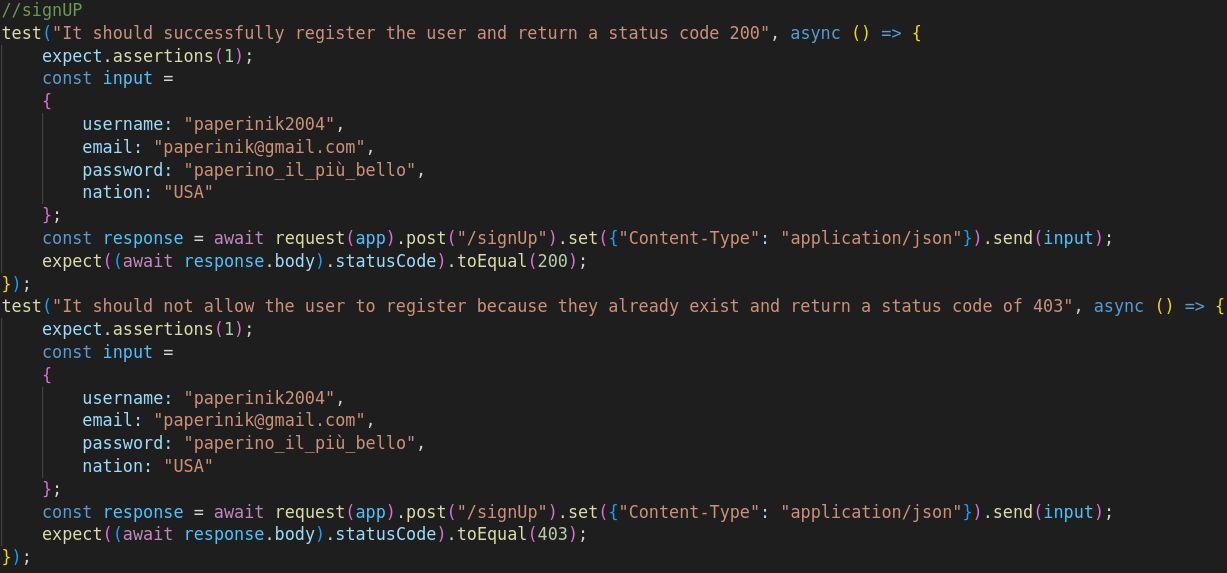
\includegraphics[scale=0.4]{images/esempio_di_test.jpg}
\caption{Esempio test API registrazione}
\label{fig:test_api}
\end{figure}
\noindent
Sono state realizzate quattro test suite, una per ogni file presente all'interno della cartella controllers:
\begin{itemize}
    \item Unlogged user API test suite: sono stati fatti tutti i test delle API che è possibile invocare se non si è loggati all'interno dell'applicazione;
    \item Logged user API test suite: sono stati fatti tutti i test delle API che è possibile invocare se si è loggati all'initerno dell'applicazione;
    \item API to generate a quiz: sono stati fatti i test dell'API che viene utilizzata per generare i quiz;
    \item API to generate a daily challenge: sono stati fatti i test dell'API che viene utilizzata per generare la sfida giornaliera.
\end{itemize}
I risultati sono stati i seguenti:

\begin{figure}[!h]
\centering
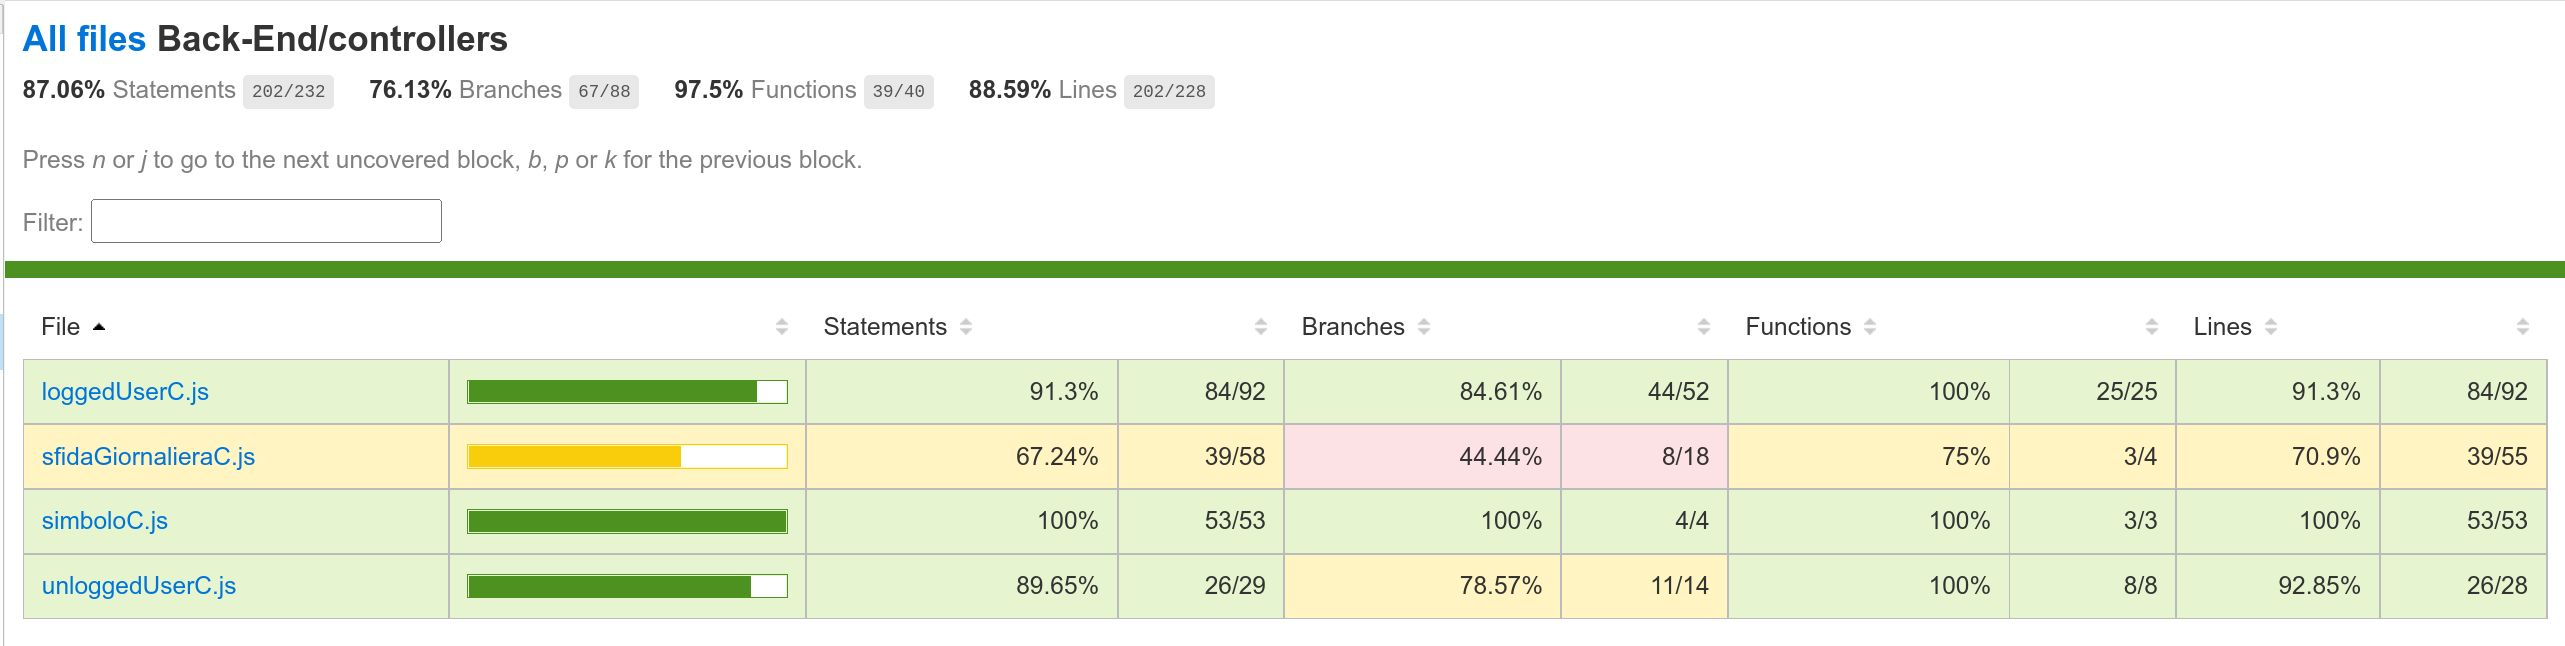
\includegraphics[scale=0.22]{images/test_result.jpg}
\caption{Rilsultato del testing}
\label{fig:test_result}
\end{figure}
\noindent
Come si può notare il file 'sfidaGiornalieraC.js' non ha avuto una gran copertura. Questo perchè ci sono due tipi di sfide giornaliere ed è possibile avere solo una sfida giornaliera per volta. Se la sfida è gia presente nel database, viene restituita quella già presente non ne viene generata una nuova ogni volta.